%! Author = Len Washington III
%! Date = 2/26/24

% Preamble
\documentclass[
	type={Programming},
	assignment={1},
	points={100},
	duedate={Sunday, March 3, 2024, 11:59 CST},
	template=true,
]{cs581homework}

% Packages

% Document
\begin{document}

\maketitle

\begin{objectives}
	\begin{enumerate}[label=\arabic*.]
		\item (100 points) Implement and evaluate two search algorithms.\\
	\end{enumerate}
\end{objectives}

\begin{inputdata}
	Your input file will be a CSV (comma-separated values) file (see Programming Assignment \#01 folder in Blackboard - campus.csv).\\

	You \underline{\textbf{CANNOT} modify nor rename} input data files.\\

	Each row in that input file will correspond to STATE information: STATE\_LABEL, and state 2D Cartesian space coordinates: $X$ and $Y$ to be positive integers.\\

	Input (four states in this case, but there will be more) file (text file) format:

	\begin{equation*}
	\begin{aligned}
		A,X_{A},Y_{A}\\
		B,X_{B},Y_{B}\\
		C,X_{C},Y_{C}\\
		D,X_{D},Y_{D}\\
	\end{aligned}
	\end{equation*}

	Where:
	\begin{itemize}
		\item $A$, $B$, $C$, $D$ are state LABELS,
		\item $X_{i}$, $Y_{i}$ are state coordinates.
	\end{itemize}
\end{inputdata}

\deliverables

\begin{problemdescription}
	You are given a weighted complete graph $G$ (example shown on Fig.~\ref{fig:hamiltonian_cycle}).
	Your task is to solve a Traveling Salesman Problem [TSP] (find minimum cost/weight Hamiltonian Cycle) on $G$ using algorithms specified below.

	\begin{figure}[H]
		\centering
		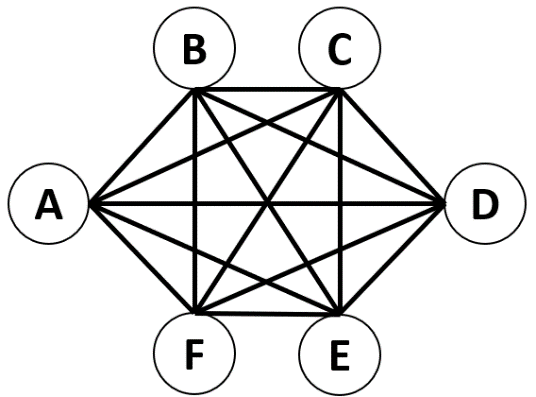
\includegraphics[width=\textwidth]{hamiltonian_cycle}
		\caption{\textit{Sample complete (fully connected, weights NOT shown graph $G$.)}}
		\label{fig:hamiltonian_cycle}
	\end{figure}

	Assume that edge weights represent \textbf{\emph{straight line distances between states}.}\\

	Your task is to implement two search algorithms in Python:
	\begin{itemize}
		\item Simulated Annealing, and
		\item Genetic Algorithm,
	\end{itemize}
	and apply them to solve the TSP (\textbf{\emph{starting at Stuart Building [SB] node}}) problem using provided data.\\
	Your program should:
	\begin{itemize}
		\item Accept four (4) command line arguments corresponding to two states / state capitals (initial and goal states) so your code could be executed with \begin{center} python cs581\_P01\_AXXXXXXXX.py FILENAME ALGO $P_{1}$ $P_{2}$ \end{center}
		where:
		\begin{itemize}
			\item cs581\_P01\_AXXXXXXXX.py is your Python code file name,
			\item FILENAME is the input CSV file name (graph $G$ data),
			\item ALGO is mode in which your program should operate
			\begin{itemize}
				\item 1 -- Simulated Annealing
				\item 2 -- Genetic Algorithm
			\end{itemize}
			\item $P_{1}$ is a value for a specific algorithm parameter:
			\begin{description}
				\item[Simulated Annealing] $P_{1}$ is the initial temperature $T$ value,
				\item[Genetic Algorithm] $P_{1}$ is the number of iterations $K$,
			\end{description}
			\item $P_{2}$ is a value for a specific algorithm parameter:
			\begin{description}
				\item[Simulated Annealing] $P_{2}$ is the \emph{$\alpha$} parameter for the temperature cooling schedule,
				\item[Genetic Algorithm] $P_{2}$ is the mutation probability $P_{m}$ value,
			\end{description}
		\end{itemize}
		Example:
		\begin{center} python cs581\_P01\_AXXXXXXXX.py DATA.csv 2 1000 0.01 \end{center}

		If the number of arguments provided is NOT four, your program should display the following error message:
		\begin{center} ERROR: Not enough or too many input arguments. \end{center} and exit.
		\item Load and process input data file provided (assume that input data file is ALWAYS in the same folder as your code - \emph{this is REQUIRED}! DO NOT HARDCODE YOUR LOCAL FILE PATH).
		Make sure your program is\\\underline{\textbf{flexible enough to accommodate different input data set}} (with a different [size, nodes, edges, etc.] graph, but structurally the same).
		\emph{Your submission will be tested using a different file!}
	\end{itemize}
\end{problemdescription}


\end{document}